\part{Mechanics}
\chapter{Kinematics}
\section{Uniformly accelerated linear motion}
\subsection{Equations of motion}
\textbf{Velocity} as function of time:
\begin{equation}
v_x(t) = v_{x0} + a_xt
\end{equation}

\begin{derivation}
For the one-dimensional case in the $x$-direction, from the definition of acceleration as the time derivative of velocity,
\[ a_x = \dv{v_x}{t} \]
Solving the differential equation,
\[ \int_{v_{x0}}^{v_x(t)} \dd{v_x} = \int_{0}^{t} a_x \dd{t} \implies v_x(t)-v_{x0} = a_xt \]

$\therefore \vb{v}(t)=(v_{x0}+a_xt)\hat{i}+(v_{y0}+a_yt)\hat{j}$
\end{derivation}

\textbf{Displacement} as function of time:
\begin{equation}
x(t)=x_0+v_{x0}t+\frac{1}{2}a_xt^2
\end{equation}

\begin{derivation}
\begin{align*}
v_x(t) &= \odv{x(t)}{t} \\
v_{x0}+a_xt &= \odv{x(t)}{t} \\
\dd{x} &= (v_{x0}+a_xt) \dd{t} \\
\int_{x_0}^{x(t)} &= \int_0^t (v_{x0}+a_xt) \dd{t} \\
x(t)-x_0 &= v_{x0}t+\frac{1}{2}a_xt^2 \\
x(t) &= x_0+v_{x0}t+\frac{1}{2}a_xt^2
\end{align*}
$\therefore \vb{r}(t)=(x_0+v_{x0}t+\frac{1}{2}a_xt^2)\hat{i}+(y_0+v_{y0}t+\frac{1}{2}a_yt^2)\hat{j}$
\end{derivation}

Eliminating time dependence:
\begin{equation}
v_x(x)^2 = {v_{x0}}^2+2a_x[x(t)-x_0]
\end{equation}

\begin{derivation}
\begin{align*}
a_x(t) &= \odv{v_x(t)}{t} \\
a_x &= \odv{v_x}{x} \odv{x}{t} \\
a_x &= v_x \odv{v_x}{x} \\
a_x \dd{x} &= v_x \dd{v_x} \\
\int_{x_0}^{x(t)}a_x\dd{x} &= \int_{v_{x0}}^{v_x(t)}v_x \dd{v_x} \\
\frac{1}{2}v_x(t)^2 - \frac{1}{2}{v_{x0}}^2 &= a_x[x(t)-x_0] \\
v_x(x)^2 &= {v_{x0}}^2+2a_x[x(t)-x_0] \\
\end{align*}
\end{derivation}

\subsection{Projectile motion}
Horizontal and vertical motions are completely \emph{independent} from each other.

Conventionally, $+x$-direction is horizontally rightward, $+y$-direction is vertically upward.

\begin{table}[H]
\centering
\begin{tabular}{cc}
\hline\hline
\textbf{Horizontal motion} & \textbf{Vertical motion} \\
\hline
$v_x(t)=v_{x0}+a_xt$ & $v_y(t)=v_{y0}+a_yt$ \\
$x(t)=x_0+v_{x0}t+\frac{1}{2}a_xt^2$ & $y(t)=y_0+v_{y0}t+\frac{1}{2}a_yt^2$ \\
$v_x(x)^2={v_{x0}}^2+2a_x(x-x_0)$ & $v_y(y)^2={v_{y0}}^2+2a_y(y-y_0)$ \\
\hline\hline
\end{tabular}
\end{table}

The trajectory of two dimensional free falling motion is given by
\begin{align*}
x(t) &= x_0+v_0\cos\theta t \implies t=\frac{x(t)-x_0}{v_0\cos\theta} \\
y(t) &= y_0+v_0\sin\theta t-\frac{1}{2}gt^2 \\
&= y_0 + \tan\theta[x(t)-x_0]-\brac{\frac{g}{2{v_0}^2\cos^2\theta}}[x(t)-x_0]^2
\end{align*}
Hence, the trajectory is \emph{parabolic}.
\pagebreak

\begin{exmp}{}{}
The acceleration of a marble in a certain fluid is proportional to the speed of the marble squared and is given by $a=-kv^2$. If the marble enters the fluid with a speed of $v_0$, how long will it take before the marble's speed is half of its initial value?
\end{exmp}

\begin{solution}
Rewriting acceleration as the derivative of velocity and solving the differential equation,
\[ a(t) = -kv(t)^2 \implies \dv{v}{t} = -kv^2 \]

Solving the differential equation,
\[ \frac{1}{v^2} \dd{v} = -k \dd{t} \implies
\int_{v_0}^{\frac{v_0}{2}} \frac{1}{v^2} \dd{v} = -\int_0^t k \dd{t} \implies
\frac{2}{v_0} - \frac{1}{v_0} = kt \implies 
\boxed{t = \frac{1}{kv_0}} \]

To determine the displacement of the marble at this time, rewrite acceleration as time derivative of velocity.
\[ \dv{v}{t} = -kv^2 \]
Using chain rule,
\[ \dv{v}{x}\dv{x}{t} = -kv^2 \]
Since $v=\dv{x}{t}$,
\[ v\odv{v}{x} = -kv^2 \]
Solving the differential equation,
\[ \frac{1}{v}\dd{v} = -k \dd{x} \implies
\int_{v_0}^{\frac{v_0}{2}}\frac{1}{v} \dd{v} = -\int_0^xk\dd{x} \implies
\ln\frac{v_0}{2}-\ln v_0 = -kx \implies
\boxed{x = \frac{\ln2}{k}} \]
\end{solution}
\pagebreak

\begin{exmp}{}{}
Ship A is 10km due west of ship B. Ship A is heading directly north at a speed of 30km/h while ship B is heading in a direction 60$\degree$ west of north at a speed of 20km/h. What will be their distance of closest approach?
\end{exmp}

\begin{solution}
We first set up a coordinate system: choose origin at initial position of ship A, $+x$-direction is eastward and $+y$-direction is northward.

Position vector of A with respect to B:
\begin{align*}
\vb{r}_{AB} &= \vb{r}_{AG} + \vb{r}_{GB} \\
&= \vb{r}_{AG} - \vb{r}_{BG} \\
&= v_At\hat{j} + (10-v_Bt\sin60\degree)\hat{i}+v_Bt\cos60\degree\hat{j} \\
&= (-10+v_B\sin60\degree t)\hat{i}+(v_At-v_B\cos60\degree t)\hat{j}
\end{align*}

Relative distance between A and B at time $t$:
\[ r_{AB} = |\vb{r}_{AB}| = \sqrt{(-10+v_B\sin60\degree t)^2+(v_At-v_B\cos60\degree t)^2} \]

To find minimum value of $r_{AB}$,
\[ \dv{r_{AB}}{t}=0 \implies t_0=\frac{\sqrt{3}}{7} \]

$\therefore$ Minimum distance between A and B = \boxed{7.56 \unit{km}}.
\end{solution}
\pagebreak

\begin{exmp}{}{}
A projectile is fired up an incline of angle $\phi$ with an initial speed $v_i$ at an angle $\theta$ with respect to the horizontal ($\theta>\phi$). Find the direction in which it should be aimed to achieve the maximum range along the incline. What is the maximum range?
\end{exmp}

\begin{solution}
$\vb{v}_x(t)=v_i\cos\theta, \vb{v}_y(t)=v_i\cos\theta$
Let the time when projectile lands on the incline be $T$.

\end{solution}
\pagebreak

\begin{exmp}{}{}
At $t=0$ on a planet, a projectile is fired with speed $v_0$ at an angle $\theta$ above the horizontal. On this planet, the acceleration due to gravity increases linearly with time, starting with a value of zero when the projectile is fired from the ground, i.e. $g(t)=\alpha t$. What horizontal distance does the projectile travel? What should $\theta$ be to maximise this distance?
\end{exmp}

\chapter{Newtonian Mechanics}
Classical mechanics is all about the motion of \textbf{particles}. We start with a definition.

\begin{defn}{Particle}{}
A particle is, loosely, defined as an object of insignificant size. 

This means that if you want to say what a particle looks like at a given time, the only information you have to specify is its position.
\end{defn}

To describe the position of a particle we need a \textbf{reference frame}. This is a choice of origin, together with a set of axes which, for now, we pick to be Cartesian. With respect to this frame, the position of a particle is specified by a vector $\vb{x}$. The trajectory of the particle with respect to time is described by
\[ \vb{x}=\vb{x}(t) \]

\begin{notation}
In this book we will use both the notation $\vb{x}(t)$ and $\vb{r}(t)$ to describe the trajectory of a particle.
\end{notation}

\begin{defn}{Velocity}{}
The \vocab{velocity} of a particle is defined to be
\begin{equation}
\vb{v} \equiv \dot{\vb{x}} = \dv{\vb{x}(t)}{t}
\end{equation}
\end{defn}

\begin{notation}
We often denote the time derivative of a variable by a dot above the variable.
\end{notation}

\begin{defn}{Acceleration}{}
The \vocab{acceleration} of the particle is defined to be
\begin{equation}
\vb{a} \equiv \ddot{\vb{x}} = \dv[2]{\vb{x}(t)}{t}
\end{equation}
\end{defn}

\subsection*{Vector Differentiation}
The derivative of a vector is defined by differentiating each of the components. For $\vb{x} = (x_1, x_2, x_3)$,
\[ \dv{\vb{x}}{t} = \brac{\dv{x_1}{t}, \dv{x_2}{t}, \dv{x_3}{t}} \]
Geometrically, the derivative of a path $\vb{x}(t)$ lies tangent to the path.

We will also be working with vector differential equations. These should be viewed as three, coupled differential equations -- one for each component. We will frequently come across situations where we need to differentiate vector dot-products and cross-products. The meaning of these is easy to see if we use the chain rule on each component. For example, given two vector functions of time, $\vb{f}(t)$ and $\vb{g}(t)$, we have
\[ \odv*{(\vb{f}\cdot\vb{g})}{t} = \dv{\vb{f}}{t}\cdot \vb{g}+\vb{f}\cdot\dv{\vb{g}}{t} \]
and
\[ \odv*{(\vb{f}\times\vb{g})}{t} = \dv{\vb{f}}{t}\times\vb{g}+\vb{f}\times\dv{\vb{g}}{t} \]

Note that the order that we write the dot product does not matter, but we have to be more careful with the cross product because, for example, 
\[ \dv{\vb{f}}{t} \times \vb{g} = -\vb{g} \times \dv{\vb{f}}{t}. \]

\section{Newton's Laws}
Newtonian mechanics is a framework which allows us to determine the trajectory $\vb{x}(t)$ of a particle in any given situation. This framework is usually presented as three axioms known as \vocab{Newton's laws of motion}. They are given by:
\begin{enumerate}[label=\textbf{N\arabic*}]
\item Left alone, a particle moves with constant velocity.
\item The acceleration (or, more precisely, the rate of change of momentum) of a particle is proportional to the force acting upon it.
\item Every action has an equal and opposite reaction.
\end{enumerate}

\section{Inertial Frames and Newton's First Law}
We have introduced the idea of a frame of reference: a Cartesian coordinate system in which you measure the position of the particle. But for reference frames such as rotating ones, for a particle of trajectory $\vb{x}(t)$, we certainly won't find that $d^2\vb{x}/dt^2=0$, i.e. particles do not travel at constant velocity.

We see that if we want Newton's first law to hold, we must be more careful about the kind of reference frames we're talking about. We first define an inertial reference frame.

\begin{defn}{Inertial reference frame}{}
An \vocab{inertial reference frame} is one in which particles travel at constant velocity when the force acting on it vanishes. 

In other words, in an inertial frame,
\[ \ddot{\vb{x}}=0 \quad \text{when} \quad \vb{F}=0 \]
\end{defn}

The true content of Newton's first law can then be better stated as: inertial frames exist.

\subsection{Galilean Relativity}
Inertial frames are not unique. Given an inertial frame $S$ in which a particle has coordinates $\vb{x}(t)$, we can always construct another inertial frame $S^\prime$ in which the particle has coordinates $\vb{x}^\prime(t)$ by any combination of the following transformations:
\begin{itemize}
\item Translation: $\vb{x}^\prime = \vb{x} + \vb{a}$, for constant $\vb{a}$.
\item Rotation: $\vb{x}^\prime = \mathbf{R}\vb{x}$, for a $3\times3$ matrix $\mathbf{R}$ obeying $\mathbf{R}^T\mathbf{R}=1$. (This also allows for reflections if $\det\mathbf{R}=-1$, although our interest will primarily be on continuous transformations).
\item Boost: $\vb{x}^\prime = \vb{x} + \vb{v}t$, for constant velocity $\vb{v}$.
\end{itemize}

\begin{remark}
The three transformations above are not quite the unique transformations that map between inertial frames. But, for most purposes, they are the only interesting ones! The others are transformations of the form $\vb{x}^\prime=\lambda\vb{x}$ for some $\lambda\in\RR$. This is just a trivial rescaling of the coordinates; for example, we can measure distances in $S$ in units of metres and distances in $S^\prime$ in units of parsecs.
\end{remark}

It is simple to prove that all of these transformations map one inertial frame to another. Suppose that a particle moves with constant velocity with respect to frame $S$, so that $d^2\vb{x}/dt^2=0$. Then, for each of the transformations above, we also have $d^2\vb{x}^\prime/dt^2=0$ which tells us that the particle also moves at constant velocity in $S^\prime$. Or, in other words, if S is an inertial frame then so too is $S^\prime$. The three transformations generate a group known as the \emph{Galilean group}.

We have already mentioned that Newton's second law is to be formulated in an \textit{inertial frame}. But, importantly, it doesn't matter which inertial frame. In fact, this is true for all laws of physics: they are the same in any inertial frame. This is known as the \textbf{principle of relativity}.

So position, direction and velocity are relative. But acceleration is not. You do not have to accelerate relative to something else. It makes perfect sense to simply say that you are accelerating or you are not accelerating. In fact, this brings us back to Newton's first law: if you are not accelerating, you are sitting in an inertial frame.

\subsection{Absolute Time}
There is one last issue that we have left implicit in the discussion above: the choice of time coordinate $t$. If observers in two inertial frames $S$ and $S^\prime$ fix the units -- seconds, minutes, hours -- in which to measure the duration time then the only remaining choice they can make is when to start the clock. In other words, the time variable in $S$ and $S^\prime$ differ only by
\[ t^\prime = t + t_0 \]

This is sometimes included among the transformations that make up the Galilean group.

The existence of a uniform time, measured equally in all inertial reference frames, is referred to as \textbf{absolute time}. It is something that we will have to revisit when we discuss special relativity. As with the other Galilean transformations, the ability to shift the origin of time is reflected in an important property of the laws of physics. The fundamental laws don't care when you start the clock. All evidence suggests that the laws of physics are the same today as they were yesterday. They are \textbf{time translationally invariant}.

\section{Newton's Second Law}
The second law is the meat of the Newtonian framework. It is the famous ``$F=ma$", which tells us how a particle's motion is affected when subjected to a force $\vb{F}$. The
correct form of the second law is
\begin{equation}
\odv*{(m\dot{\vb{x}})}{t} = \vb{F}(\vb{x},\dot{\vb{x}})
\end{equation}
This is usually referred to as the equation of motion. The quantity in brackets is called the \vocab{momentum}:
\[ \vb{p} \equiv m\dot{\vb{x}} \]
where $m$ is the (inertial) mass of the particle.

In cases where mass does not change with time, we can write the second law in the more familiar form:
\begin{equation}
m\ddot{\vb{x}} = \vb{F}(\vb{x},\dot{\vb{x}})
\end{equation}

Newton's equation is a second order differential equation; this means that we will have a unique solution only if we specify two initial conditions. These are usually taken to be the position $\vb{x}(t_0)$ and the velocity $\dot{\vb{x}}(t_0)$ at some initial time $t_0$.

\chapter{Forces}
\section{Potentials in One Dimension}
Consider a particle with position function $x(t)$. For now, suppose that the force on the particle depends only on its position, not its velocity: $F=F(x)$. We define the \vocab{potential} $V(x)$ (also called the potential energy) by the equation
\begin{equation}\label{potential}
F(x) = -\dv{V}{x}
\end{equation}

The potential is only defined up to an additive constant. We can always invert \cref{potential} by integrating both sides. The integration constant is now determined by the choice of lower limit of the integral:
\[ V(x) = -\int_{x_0}^x F(x^\prime) \dd{x^\prime} \]
where $x^\prime$ is just a dummy variable.

With this definition, we can write the equation of motion as
\begin{equation}\label{conservative}
m\ddot{x} = -\dv{V}{x}
\end{equation}

For any force in one-dimension which depends only on the position, there exists a \emph{conserved} quantity called the \vocab{energy},
\[ E = \frac{1}{2}m\dot{x}^2 + V(x) \]

The fact that this is conserved means that $\dot{E} = 0$ for any trajectory of the particle which obeys the equation of motion. While $V(x)$ is called the potential energy, $T=\frac{1}{2}m\dot{x}^2$ is called the \vocab{kinetic energy}. Motion satisfying \cref{conservative} is called \vocab{conservative}.

It is not hard to prove that $E$ is conserved. We need only differentiate with respect to time to get
\[ \dot{E} = m\dot{x}\ddot{x} + \dv{V}{x}\dot{x} = \dot{x}\brac{m\ddot{x}+\dv{V}{x}} = 0 \]
where the last equality holds courtesy of the equation of motion \cref{conservative}.

\subsection{Uniform Gravitational Field}
In a uniform gravitational field, a particle is subjected to a constant force, $F=-mg$ where $g \approx 9.8$  \unit{ms^{-2}} is the acceleration due to gravity near the surface of the Earth. The minus sign arises because the force is downwards while we have chosen to measure position in an upwards direction, which we call $z$. The potential energy is
\begin{equation}
V = mgz
\end{equation}

\begin{remark}
Notice that we have chosen to have $V=0$ at $z=0$. There is nothing that forces us to do this; we could easily add an extra constant to the potential to shift the zero to some other height.
\end{remark}

The equation of motion for uniform acceleration is
\[ \ddot{z}=-g \]
Which can be integrated to give the velocity at time $t$,
\[ \dot{z} = u - gt \]
where $u$ is the initial velocity at time $t=0$.

Integrating once more gives the position
\[ z = z_0 + ut - \frac{1}{2}gt^2 \]
where $z_0$ is the initial height at time $t=0$.

\subsection{Harmonic Oscillator}
The potential energy of the harmonic oscillator is defined to be
\[ V(x) = \frac{1}{2}kx^2 \]

The force resulting from the energy $V$ is given by $F=-kx$ which, in the context of the spring, is called \vocab{Hooke's law}. The equation of motion is
\begin{equation}
m\ddot{x} = -kx
\end{equation}
which has the general solution
\[ x(t) = A \cos(\omega t) + B \sin(\omega t) \quad \text{with }\omega=\sqrt{\frac{k}{m}} \]
where $A$ and $B$ are two integration constants and $\omega$ is called the angular frequency. The coefficients $A$ and $B$ determine the amplitude of the oscillations, together with the phase at which you start the cycle. The time taken to complete a full cycle is called the period
\begin{equation}
T = \frac{2\pi}{\omega}
\end{equation}
The period is independent of the amplitude.

If we want to determine the integration constants A and B for a given trajectory, we need some initial conditions. For example, if we're given the position and velocity at time $t=0$, then it's simple to check that $A=x(0)$ and $B=\frac{\dot{x}(0)}{\omega}$.

\subsection{Moving in a Potential}


\chapter{Translational Dynamics}
\section{Forces}
\subsection{Types of forces}
\subsubsection{Weight}
Weight $\vb{W}$ is the gravitational force exerted by Earth on an object.

\subsubsection{Normal force}
Normal force $\vb{N}$ is the contact force exerted by a surface (ground or floor) on an object.

\subsubsection{Tension force}
Tension force $\vb{T}$ is the force experienced in an object when it is deformed (compressed or depressed).

\subsubsection{Spring force}
\begin{thrm}{Hooke's Law}{}
Spring force is directly proportional to extension of spring.
\begin{equation}
\vb{F}_s = -k\vb{x}
\end{equation}
where $k$ is the spring constant.
\end{thrm}

\subsubsection{Frictional force}
There are two types of frictional force:
\begin{itemize}
\item \textbf{Kinetic friction force}: object is sliding on rough surface
\[ f_k = \mu_k N \]
\item \textbf{Static friction force}: object is not sliding
\[ f_s \le \mu_s N \]
\end{itemize}

\subsubsection{Resistive force}
Drag force $F_R$: force caused by interaction of an object and the fluid it is moving through
\begin{itemize}
\item For objects moving at low speeds: resistive force is directly proportional to speed
\begin{equation}
\vb{F}_R = -b\vb{v}
\end{equation}

\item For objects moving at high speeds: resistive force is directly proportional to square of speed
\begin{equation}
\vb{F}_R = -\frac{1}{2}D\rho A\vb{v}^2
\end{equation}
where $D$ is the drag coefficient, which depends on the shape and surface texture of the object.

\textbf{Terminal velocity} is when an object moving through a fluid has reached translational equilibrium. For an object falling downwards:
\[ \sum \vb{F}_y = \vb{F}_g-\vb{F}_R = m\vb{a}_y \implies mg-\frac{D}{\rho}Av^2 = ma_y \implies a_y = g-\frac{D\rho Av^2}{2m} \]
In absence of air resistance, $\vb{a}_y=g$.

When $\vb{a}_y=0$,
\[ \frac{D\rho Av^2}{2m} = g \implies \boxed{v_\text{terminal} = \sqrt{\frac{2mg}{D\rho A}}} \]
\end{itemize}
\pagebreak

\section{Centre of mass}
\begin{defn}{Centre of mass}{}
A special point in a system, as if all of the mass of the system is concentrated at that point. 
\end{defn}

Centre of mass for a \textbf{system of point particles}:
\begin{equation}
x_{CM} = \frac{\sum_i m_i x_i}{\sum_i m_i} \quad 
y_{CM} = \frac{\sum_i m_i y_i}{\sum_i m_i} \quad
z_{CM} = \frac{\sum_i m_i z_i}{\sum_i m_i}
\end{equation}
where the distances depend on the \emph{coordinate system} set up.

Centre of mass of an \textbf{extended object} (think of an extended object as a system containing infinitely many small mass elements):
\[ x_{CM} = \lim_{\Delta m_i \to 0} \frac{1}{M} \sum_i x_i \Delta m_i \]
\begin{equation}
x_{CM} = \frac{1}{M} \int x \dd{m} \quad
y_{CM} = \frac{1}{M} \int y \dd{m} \quad
z_{CM} = \frac{1}{M} \int z \dd{m}
\end{equation}

\subsection{Motion of centre of mass}
\subsubsection{Velocity}
$x$-, $y$- and $z$-components of the velocity of centre of mass, denoted by $v_{CM,x}$, $v_{CM,y}$ and $v_{CM,z}$, are the time derivatives of $x_{CM}$, $y_{CM}$ and $z_{CM}$ respectively.
\begin{equation}
v_{CM,x} = \frac{\sum_i m_i v_{xi}}{\sum_i m_i} \quad 
v_{CM,y} = \frac{\sum_i m_i v_{yi}}{\sum_i m_i} \quad
v_{CM,z} = \frac{\sum_i m_i v_{zi}}{\sum_i m_i}
\end{equation}

These equations can be written as one single vector equation:
\begin{equation}
\vb{v}_{CM} = \frac{1}{M}\sum_{i}m_i\vb{v}_i
\end{equation}

Total momentum of the system is given by
\begin{equation}
\vb{p} = M\vb{v}_{CM} = \sum_{i}m_i\vb{v}_i
\end{equation}
This equation states that the total momentum is the product of total mass and velocity of centre of mass.

\subsubsection{Acceleration and external force}
Taking time derivative of the above equation gives
\[ M\vb{a}_{CM} = \sum_{i}m_i\vb{a}_i \]

Note that $\sum_{i}m_i\vb{a}_i$ is simply the sum of all forces (external and internal):
\[ \sum\vb{F} = \sum\vb{F}_{ext} + \sum\vb{F}_{int} = \sum_{i}m_i\vb{a}_i \]

By Newton's 3rd law, internal forces all cancel in pairs so $\sum\vb{F}_{int}=0$. Hence
\begin{equation}
\sum\vb{F}_{ext} = M\vb{a}_{CM} \quad \text{and} \quad \sum\vb{F}_{ext}=\odv{\vb{p}}{t}
\end{equation}

When a body or a collection of particles is acted on by external forces, centre of mass moves as though all the mass were concentrated at that point and it were acted on by a net force equal to the sum of external forces on the system.

For example, a shell explodes into two fragments in flight. Ignoring air resistance, centre of mass continues on the same trajectory aas the shell's path before exploding.
\begin{figure}[H]
    \centering
    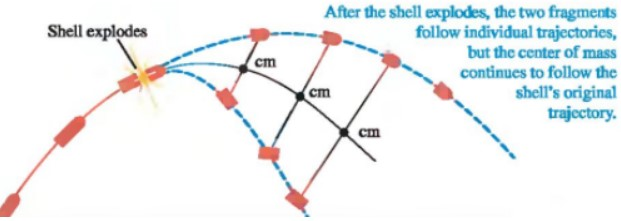
\includegraphics{images/shell_explode_cm.jpg}
\end{figure}

Note that if the net external force acting on the system is zero, we get
\[ \dv{\vb{p}}{t}=0 \implies M\vb{v}_{CM}=\vb{p}=\text{constant} \]
\pagebreak

\section{Equilibrium}
Equilibrium conditions: 
\begin{enumerate}
\item force balance (vectorially or in terms of projections)
\item torque balance (only for one- and two-dimensional geometry). 
\end{enumerate}

Stable and unstable equilibria.
\pagebreak

\section{Elastic modulus}
compression.
We consider three types of deformation and define an elastic modulus for each:
\begin{enumerate}
\item \textbf{Young's modulus} measures the resistance of a solid to a change in its length.
\item \textbf{Shear modulus} measures the resistance to motion of the planes within a solid parallel to each other.
\item \textbf{Bulk modulus} measures the resistance of solids or liquids to changes in their volume.
\end{enumerate}

\subsection{Tensile and compressive}
We usually assume objects to be rigid. When large forces are applied to an object, it deforms. 

Suppose that we pull on the ends of a bar with a force $F$. We say that the bar is in tension. The internal forces in the bar resist the tension forces and hold the bar together. Even so, the bar deforms and the equilibrium length of the bar increases. 

If the bar is in equilibrium with the applied forces, then every cross section of the bar must be subject to the same internal forces that resist stretching.

\begin{defn}{Stress}{}
Ratio of the magnitude of the applied force $F$ to cross-sectional area $A$.
\begin{equation}
\sigma \equiv \frac{F}{A}
\end{equation}
\end{defn}

\begin{remark}
There are two types of stress: tensile and compressive.
\end{remark}

\begin{defn}{Strain}{}
Ratio of the change in length $\delta$ to the initial length $L$.
\begin{equation}
\varepsilon \equiv \frac{\delta}{L}
\end{equation}
\end{defn}

\begin{remark}
There are two types of strain: tensile and compressive.
\end{remark}

The amount of strain an object undergoes depends on the stress applied to it. If the stress is not too great, the strain is observed to be proportional to the stress.

\begin{defn}{Young modulus}{}
Ratio of stress to strain.
\begin{equation}
Y \equiv \frac{\sigma}{\varepsilon} = \frac{FL}{A\delta}
\end{equation}
\end{defn}

\subsection{Shear}
When an external force acts on an object, it undergoes deformation. If the direction of the force is parallel to the plane of the object. The deformation will be along that plane. The stress experienced by the object here is shear stress.

\begin{defn}{Shear stress}{}
A type of stress that acts coplanar with cross section of material.
\begin{equation}
\tau \equiv \frac{F}{A}
\end{equation}
\end{defn}

Shear stress arises due to shear forces. They are the pair of forces acting on opposite sides of a body with the same magnitude and opposite direction. 
\pagebreak

\section{Work Done and Energy}
\subsection{Work}
Work done by a constant force:
\begin{equation}
W = \vb{F} \cdot \Delta\vb{r} = F\Delta r\cos\theta
\end{equation}
where $\theta$ is the angle between $\vb{F}$ and $\vb{r}$.

Work done by a non-constant force:
\begin{equation}
W = \int_{x_i}^{x_f}F_x \dd{x}
\end{equation}

\subsection{Energy}
\begin{thrm}{Net Work -- Kinetic Energy Theorem}{}
\begin{equation}
\sum W = \Delta K
\end{equation}
\end{thrm}

Kinetic energy for translational motion:
\begin{equation}
K=\frac{1}{2}mv^2
\end{equation}

Gravitational potential energy (in constant gravitational field):
\begin{equation}
U_g = mgh
\end{equation}

Potential energy for simple force fields (also as a line integral of the force field). 


Relationship between conservative forces and potential energy:
\begin{equation}
F = -\dv{U}{x}
\end{equation}


\subsection{Power}
\begin{defn}{Power}{}
Rate at which work is done
\begin{equation}
P_\text{avg} = \frac{W}{\Delta t}
\end{equation}
\begin{equation}
P_\text{instantaneous} = \dv{W}{t}
\end{equation}
\end{defn}

Instantaneous power (constant force):
\begin{equation}
P_\text{instantaneous} = \vb{F} \cdot \vb{v}
\end{equation}
\begin{derivation}
\[ P_\text{instantaneous} = \dv{W}{t} = \dv{(\vb{F}\cdot\Delta\vb{r})}{t} = F \cdot \dv{\Delta\vb{r}}{t} = \vb{F}\cdot\vb{v} \]
\end{derivation}

\pagebreak

\chapter{Rotational Motion}
\section{Kinematics}
\begin{defn}{Radian}{}
\begin{equation}
\theta \equiv \frac{s}{r}
\end{equation}
\end{defn}

\begin{defn}{Angular displacement}{}
The angle that a rigid object rotates through during some time interval.
\begin{equation}
\Delta \theta \equiv \theta_f - \theta_i
\end{equation}
\end{defn}

\begin{remark}
Every point on a rigid object undergoes the same angular displacement in any given time interval.
\end{remark}

\begin{defn}{Angular velocity}{}
Rate of change of angular displacement with respect to time.
\begin{equation}
\omega(t) \equiv \lim_{\Delta t \to 0} \frac{\Delta \theta}{\Delta t} = \dv{\theta (t)}{t}
\end{equation}
\end{defn}

\begin{remark}
Every part of a rotating rigid object has the same angular velocity at any instant of time.
\end{remark}

Direction of angular velocity can be found using the ``right hand rule". Curl fingers of right hand around rotation. Thumb points in the direction of the vector.

\begin{defn}{Angular acceleration}{}
Rate of change of angular velocity with respect to time.
\begin{equation}
\alpha (t) \equiv \lim_{\Delta t \to 0} \frac{\Delta \omega}{\Delta t} = \odv{\omega (t)}{t} = \odv{^2 \theta (t)}{t}
\end{equation}
\end{defn}

\textbf{Angular velocity} as a function of time 
\begin{equation}
\omega(t) = \omega_0 + \alpha t
\end{equation}

\textbf{Angular position} as a function of time
\begin{equation}
\theta(t) = \theta_0 + \omega_0 t + \frac{1}{2}\alpha t^2
\end{equation}

Eliminating time dependence
\begin{equation}
\omega^2(t) = {\omega_0}^2 + 2 \alpha [\theta (t) - \theta_0]
\end{equation}

For constant $a$ and $\alpha$, we can write analogous equations for rotational motion as in linear motion, as shown above.

\textbf{Tangential velocity} (linear speed):
\begin{equation}
v = r\omega
\end{equation}

\begin{derivation}
\[ v = \odv{s}{t} = \odv{(r\theta)}{t} = r\odv{\theta}{t} = r\omega \]
\end{derivation}

\textbf{Tangential acceleration}:
\begin{equation}
a_t = r \alpha
\end{equation}
\begin{derivation}
\[ a_t = \odv{v}{t} = \odv{(r\omega)}{t} = r\odv{\omega}{t} = r\alpha \] 
\end{derivation}

\textbf{Centripetal acceleration}
\begin{equation}
a_r = \frac{v^2}{r} = r\omega^2
\end{equation}
\begin{derivation}
\begin{align*}
\frac{\Delta v}{v} &= \frac{\Delta s}{r} \\
\Delta v &= \frac{v}{r} \Delta s \\
\lim_{\Delta t \to 0} \frac{\Delta v}{\Delta t} &= \frac{v}{r} \lim_{\Delta t \to 0} \frac{\Delta s}{\Delta t}
\end{align*}
\end{derivation}

Acceleration is the vector sum of tangential acceleration and centripetal acceleration.
\[ \vb{a} = \vb{a_t} + \vb{a_r} \]
\begin{equation}
|\vb{a}| = \sqrt{{a_t}^2 + {a_r}^2} = r \sqrt{\alpha^2 + \omega^4}
\end{equation}

Comparison between translational and rotational motion:
\begin{table}[H]
\centering
\begin{tabular}{|c|c|c|}
\hline
Quantity & Translational & Rotational \\
\hline
Displacement & $x$ & $\theta$ \\
Velocity & $v$ & $\omega$ \\
Acceleration & $a$ & $\alpha$ \\
Mass / moment of inertia & $m$ & $I$ \\
Momentum & $p$ & $L$ \\
\hline
\end{tabular}
\end{table}
\pagebreak

\section{Dynamics}
\subsection{Moment of Inertia}
Moment of inertia is the measure of the resistance of an object to changes in its rotational motion, depends on the \underline{choice of rotational axis}.

Moment of inertia of one particle:
\begin{equation}
I \equiv mr^2
\end{equation}

Moment of inertia of a system of particles:
\begin{equation}
I = \sum_i m_i {r_i}^2
\end{equation}

Moment of inertia of a continuous rigid object (divide it into infinitely many small elements):
\[ I = \lim_{\Delta m_i \to 0} \sum_i {r_i}^2 \Delta m_i \]
\begin{equation}
I = \int r^2 \dd{m}
\end{equation}

Moments of inertia of homogeneous rigid objects:\footnote{Memorise these important ones.}
\begin{table}[H]
\centering
\renewcommand{\arraystretch}{2.0}
\begin{tabular}{|c|c|}
\hline
\textbf{Object} & \textbf{Moment of inertia} \\
\hline
Hoop about central axis & $I=MR^2$ \\
Solid cylinder (or disk) about central axis & $I=\dfrac{1}{2}MR^2$ \\
Solid cylinder (or disk) about central diameter & $I=\dfrac{1}{4}MR^2+\dfrac{1}{12}ML^2$ \\
Thin rod about axis through center perp to length & $I=\dfrac{1}{12}ML^2$ \\
Solid sphere about any diameter & $I=\dfrac{2}{5}MR^2$ \\
Thin spherical shell about diameter & $I=\dfrac{2}{3}MR^2$ \\
Hoop about any diameter & $I=\dfrac{1}{2}MR^2$ \\
\hline
\end{tabular}
\end{table}

Expressions for \textbf{mass densities} come in useful:
\[ \dd{m} = \begin{cases}
    \lambda \dd{x} & \text{linear mass density} \\
    \sigma \dd{x} & \text{surface mass density} \\
    \rho \dd{x} & \text{volume mass density}
\end{cases} \]
\pagebreak

\begin{exmp}{}{}
Moment of inertia of a uniform thin hoop of mass $M$ and radius $R$ about an axis perpendicular to the plane of the hoop and passing through its center.
\end{exmp}

\begin{solution}
For constant radius, moment of inertia is given by
\[ I = \int r^2 \dd{m} = R^2 \int \dd{m} = \boxed{MR^2} \]
\end{solution}

\begin{exmp}{}{}
Moment of inertia of a uniform rigid rod of length $L$ and mass $M$ about an axis perpendicular to the rod and passing through its centre of mass.
\end{exmp}

\begin{solution}
Set up coordinate system: rod lies along $x$-axis, axis lies along $y$-axis.

A small length $\dd{x}$ at a distance $x$ from origin has a mass $\dd{m}$. Let $\lambda$ be \textbf{linear mass density}, then
\[ \lambda = \frac{M}{L} = \odv{m}{x} \implies \dd{m} = \frac{M}{L} \dd{x} \]

Moment of inertia is given by
\[ I = \int r^2 \dd{m} = \int x^2 \frac{M}{L} \dd{x} = \frac{M}{L} \int_{\frac{L}{2}}^{\frac{L}{2}} x^2\dd{x} = \frac{M}{L}\sqbrac{\frac{2}{3}\brac{\frac{L}{2}}^3} = \boxed{\frac{1}{12}ML^2} \]
\end{solution}

\begin{exmp}{}{}
Moment of inertia of uniform solid cylinder has a radius $R$, mass $M$ and length $L$ about its axis of cylinder.
\end{exmp}

\begin{solution}
The solid cylinder has to be cut or split into infinitesimally thin rings. Each ring consists of the thickness of $\dd{r}$ with length $L$. We then sum up the moments of these infinitesimally thin cylindrical shells. 

Using the concept of volume mass density $\rho$,
\[ \dd{m} = \rho \dd{V} = \rho (L \dd{A}) = \rho L (\pi(r+\dd{r})^2 - \pi r^2) = (2\pi r)L\rho\dd{r} \]

Moment of inertia is given by
\[ I = \int r^2 \dd{m} = \int_0^R2\pi r^3 L\rho \dd{r} = 2\pi L\rho \int_0^R r^3 \dd{r} = \frac{1}{2}(\pi r^2L\rho)R^2 = \boxed{\frac{1}{2}MR^2} \]
\end{solution}

\begin{exmp}{}{}
Moment of inertia of a solid sphere of mass $M$ and radius $R$ about an axis through its centre.
\end{exmp}

\begin{solution}
The expression for the moment of inertia of a sphere can be developed by summing the moment of infinitely thin disks about the $z$-axis through its centre.

\begin{figure}[H]
    \centering
    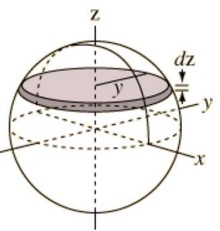
\includegraphics[width=5cm]{images/moi_sphere.jpg}
\end{figure}

Using volume mass density:
\[ \rho = \frac{M}{V} = \dv{m}{V} \implies \dd{m} = \rho\dd{V} \]

Moment of inertia of one disk about $z$-axis:
\[ \dd{I} = \frac{1}{2}y^2\dd{m} = \frac{1}{2}y^2\rho\dd{V} = \frac{1}{2}y^2\rho\pi y^2\dd{z} \]

Hence moment of inertia of sphere about $z$-axis is given by
\[ I_{CM} = \int \dd{I} = \frac{1}{2}\rho\pi\int_{-R}^R y^4\dd{z} = \frac{1}{2}\rho\pi\int_{-R}^R (R^2-z^2)^2\dd{z} = \frac{8}{15}\rho\pi R^5 = \boxed{\frac{2}{5}MR^2} \]

\begin{remark}
Another method is to sum up spherical hollow shells.
\end{remark}
\end{solution}

\begin{exmp}{}{}
Moment of inertia of a hollow cylinder with inner radius $R_1$ and outer radius $R_2$ about the central axis.
\end{exmp}

\begin{figure}[H]
    \centering
    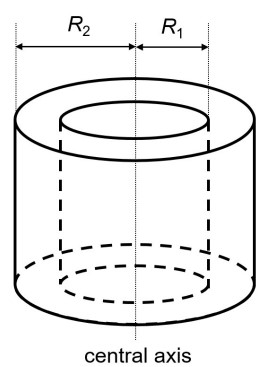
\includegraphics[width=5cm]{images/moi_hollow_cylinder.jpg}
\end{figure}

\begin{proof}
Consider a hollow cylindrical shell with radius $r$ and height $L$.

Using volume mass density,
\[ \rho=\dv{m}{V} \implies \dd{m}=\rho\dd{V} = 2\pi\rho Lr \dd{r} \]

Hence moment of inertia is 
\[ I = \int r^2\dd{m} = \int_{R_\text{in}}^{R_\text{out}} 2\pi\rho Lr^3 \dd{r} = \frac{\pi\rho L}{2}\sqbrac{r^4}_{R_\text{in}}^{R_\text{out}} = \boxed{\frac{1}{2}M(R_\text{out}^2+R_\text{in}^2)} \]
where $\rho = \dfrac{M}{\pi(R_\text{out}^2-R_\text{in}^2)L}$.
\end{proof}
\pagebreak

\begin{thrm}{Parallel axis theorem}{}
Moment of inertia $I$ about any axis parallel to axis through CM and a distance $D$ away is given by
\begin{equation}
I = I_{CM} + MD^2
\end{equation}
\end{thrm}

\begin{figure}[H]
    \centering
    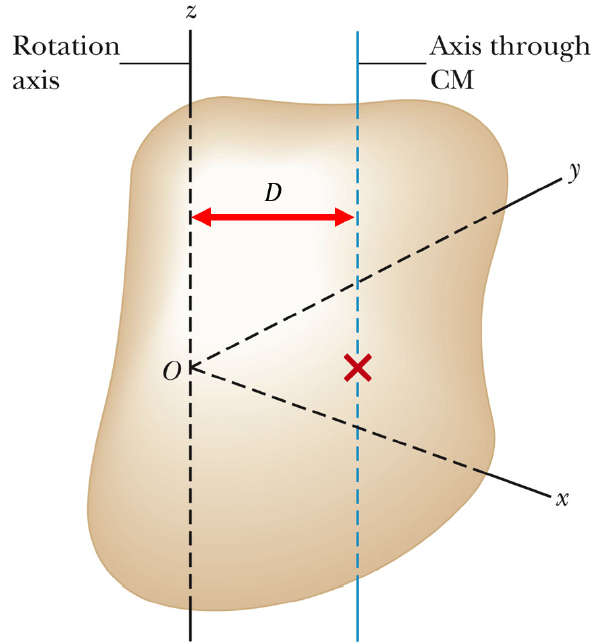
\includegraphics[width=7cm]{images/Parallel_axis_theorem.png}
    \caption{Parallel axis theorem}
\end{figure}

\begin{proof}
Moment of inertia about the $z$-axis is 
\[ I=\int r^2 \dd{m} = \int (x^2+y^2)\dd{m} \]
From the figure, $x=x^\prime+x_{CM}$ and $y=y^\prime+y_{CM}$ hence
\begin{align*}
I &= \int \left[(x^\prime+x_{CM})^2 + (y^\prime+y_{CM})^2\right] \dd{m} \\
&= \int (x^{\prime 2}+y^{\prime 2}) \dd{m} + ({x_{CM}}^2+{y_{CM}}^2) \int \dd{m} + 2x_{CM} \int x^\prime \dd{m} + 2y_{CM} \int y^\prime \dd{m}
\end{align*}
By definition of centre of mass, $\int x^\prime \dd{m} = \int y^\prime \dd{m} = 0$.

Given that $\int\dd{m}=M$ and $D^2={x_{CM}}^2+{y_{CM}}^2$,
\[ \boxed{I=I_CM+MD^2} \]
\end{proof}
\begin{figure}[H]
    \centering
    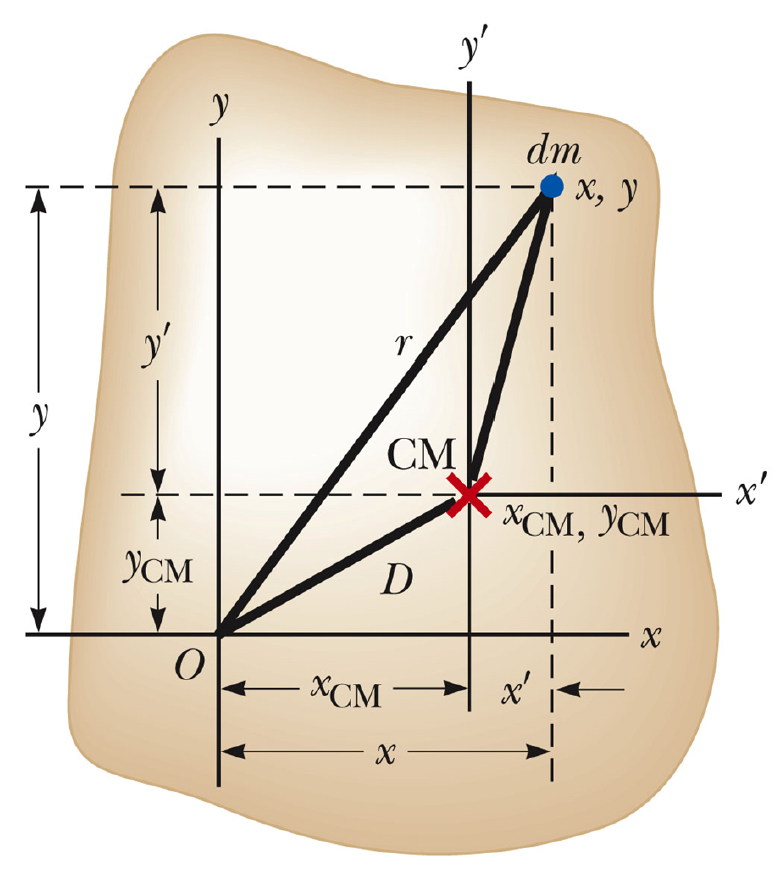
\includegraphics[width=7cm]{images/Parallel_axis_theorem2.png}
\end{figure}

\begin{exmp}{}{}
Consider a uniform rigid rod of mass $M$ and length $L$. Find the moment of inertia of the rod about an axis perpendicular to the rod through one end.
\end{exmp}

\begin{solution}
Moment of inertia is 
\[ \frac{1}{12}ML^2 + M\brac{\frac{L}{2}}^2 = \boxed{\frac{1}{3}ML^2} \]
\end{solution}

\begin{thrm}{Perpendicular axis theorem}{}
Sum of moments of inertia about any two perpendicular axes in the plane of the body is equal to the moment of inertia about an axis through the point of intersection, perpendicular to the plane of the object.
\begin{equation}
I_z = I_x + I_y
\end{equation}
This theorem works only for planar figures (2D bodies), i.e. bodies of negligible thickness.
\end{thrm}

\begin{proof}
\begin{align*}
I_z &= \int r^2 \dd{m} \\
&= \int (x^2+y^2) \dd{m} \\
&= \int x^2 \dd{m} + \int y^2 \dd{m} \\
\end{align*}
\end{proof}
\pagebreak

\subsection{Rotational kinetic energy}
We treat a rigid object as a collection of particles rotating about a fixed $z$-axis with an angular speed $\omega$.

Kinetic energy of the $i$-th particle is given by 
\[ K_i = \frac{1}{2} m_i {v_i}^2 = \frac{1}{2} m_i (r_i \omega)^2 = \frac{1}{2} m_i {r_i}^2 \omega^2 \]

Hence rotational kinetic energy possessed by a rigid object is given by 
\[ K = \sum_i K_i = \frac{1}{2}\left( \sum_i m_i {r_i}^2 \right) \omega^2 \]
\begin{equation}
K = \frac{1}{2} I \omega^2
\end{equation}

\begin{remark}
Notice the similarities between this and the formula for translational kinetic energy $K=\frac{1}{2}mv^2$.
\end{remark}
\pagebreak

\subsection{Torque}
\begin{defn}{Torque}{}
The measure of tendency of a force to \emph{rotate} an object about some axis.
\end{defn}

\begin{equation}
|\vb{\tau}| = F\ell = F\cdot r\sin\theta
\end{equation}
where $\ell = r\sin\theta$ is the \textbf{level arm}, i.e. the perpendicular distance from axis of rotation to the line of action of force.

Representing torque as a vector,
\begin{equation}
\mathbf{\tau} = \vb{r} \times \vb{F}
\end{equation}

\subsubsection{Torque and angular acceleration}
\begin{equation}
\vb{\tau} = I\alpha
\end{equation}
\begin{proof}
Consider a force $\dd{\vb{F}}_t$ acting on a mass element $\dd{m}$ of an extended object. 

From Newton's 2nd law,
\[ \dd{\vb{F}}_t = (\dd{m})a_t \implies d\vb{\tau} = r\dd{\vb{F}}_t = ra_t\dd{m} \]
Since $a_t=r\alpha$,
\[ \dd{\vb{\tau}} =  \alpha r^2\dd{m} \]
Net torque about origin due to all external forces is 
\[ \sum\vb{\tau} = \int\dd{\vb{\tau}} = \int\alpha r^2\dd{m} = \alpha\int r^2\dd{m} = \boxed{I\alpha}  \]
\end{proof}
\pagebreak

\subsection{Work, Energy, Power}
The work done by force $F$ on an object as it rotates through an infinitesimal distance $\dd{s}=r\dd{\theta}$ is
\[ \dd{W} = F\dd{s} = (F\sin\phi)r\dd{\theta} = \tau\dd{\theta} \]
Integrating both sides gives
\begin{equation}
W = \int \vb{\tau} \dd{\theta}
\end{equation}

Rate at which work is done by $F$ as the object rotates about the fixed axis through an angle $\dd{\theta}$ in a time interval $\dd{t}$ is
\[ \odv{W}{t} = \tau\odv{\theta}{t} \]
Hence power is
\begin{equation}
P=\tau\omega
\end{equation}

\begin{thrm}{Work--kinetic energy theorem}{}
Net work done by external forces in rotating a rigid body about a fixed axis equals the change in the object's rotational kinetic energy.
\begin{equation}
\sum W = \frac{1}{2}I\omega_f^2 - \frac{1}{2}I\omega_i^2
\end{equation}
\end{thrm}
\pagebreak

\subsection{Rolling motion}
In pure rolling motion, an object rolls without slipping. 

The object rotates through an angle $\theta$, so centre of mass moves a linear distance $s=R\theta$. 

Linear speed of centre of mass:
\begin{equation}
v_{CM} = R\omega
\end{equation}
\begin{derivation}
\[ v_{CM} = \odv{s}{t} = R\odv{\theta}{t} = R\omega \]
\end{derivation}

Linear acceleration of centre of mass:
\begin{equation}
a_{CM} = R\alpha
\end{equation}
\begin{derivation}
\[ a_{CM} = \odv{v_{CM}}{t} = R\odv{\omega}{t} = R\alpha \]
\end{derivation}

\textbf{Pure rolling motion} is a combination of 
\begin{itemize}
\item pure \textbf{translational motion} of centre of mass
\item pure \textbf{rotational motion} around centre of mass
\end{itemize}

Total kinetic energy of a rolling object is the \textbf{sum} of rotational kinetic energy about centre of mass and translational kinetic energy of centre of mass.
\begin{equation}
K = \frac{1}{2}I_{CM}\omega^2 + \frac{1}{2}M{v_{CM}}^2
\end{equation}
\begin{derivation}
Object rotates about point $P$, the point of contact with ground.

Total kinetic energy can be expressed as
\[ K=\frac{1}{2}I_P\omega^2 \]
where $I_P$ is the moment of inertia about an axis through $P$.

Using parallel axis theorem,
\[ I_P = I_{CM} + MR^2 \]

Hence 
\[ K = \frac{1}{2}I_{CM}\omega^2 + \frac{1}{2}M(R\omega)^2 = \boxed{\frac{1}{2}I_{CM}\omega^2 + \frac{1}{2}Mv_{CM}^2} \]
\end{derivation}
\pagebreak

\subsection{Angular momentum}
\begin{defn}{Angular momentum}{}
Cross product of instantaneous position vector $\vb{r}$ and linear momentum $\vb{p}$.
\begin{equation}
L \equiv \vb{r} \times \vb{p}
\end{equation}
\end{defn}

\begin{derivation}
From the definition of torque, $\vb{\tau} \equiv \vb{r}\times\vb{F}$,
\[ \sum\vb{\tau} = \vb{r}\times\sum\vb{F} = \vb{r}\times\odv{\vb{p}}{t} \]
Add the term $\odv{\vb{r}}{t}\times\vb{p}$ to the right-hand side, which is zero because $\odv{\vb{r}}{t}=\vb{v}$ which is parallel to $\vb{p}$.
\[ \sum\vb{\tau} = \vb{r}\times\odv{\vb{p}}{t} + \dv{\vb{r}}{t}\times\vb{p} = \dv{(\vb{r}\times\vb{p})}{t} = \boxed{\dv{\vb{L}}{t}} \]
\end{derivation}

Hence the torque acting on a particle is equal to the time rate of change of angular momentum.
\begin{equation}
\sum\mathbf{\tau} = \dv{\vb{L}}{t}
\end{equation}
This is the rotational analog of Newton's 2nd law.

\subsubsection{System of particles}
Total angular momentum of a system of particles about some point is defined as the vector sum of angular momentum of the individual particles.
\[ L_{total} = \sum_i L_i \]
Hence
\[ \sum_i \tau_i = \sum_i \odv{L_i}{t} = \odv{L_{total}}{t} \]

The torque acting on the particles of the system are due to internal forces between particles and external forces. However, net torque due to internal forces is zero as a result of Newton's 3rd law. Hence total angular momentum of system varies only if net external torque acts on the system:
\begin{equation}
\sum\mathbf{\tau}_\text{ext} = \dv{\vb{L}}{t}
\end{equation}

Net torque about axis through origin equals time rate of change of total angular momentum of system about that origin.

\begin{thrm}{}{}
Resultant torque acting on a system about axis through \underline{centre of mass} equals time rate of change of angular momentum \underline{regardless of motion of centre of mass}.
\end{thrm}

\subsubsection{Rigid body}
Angular momentum of one particle is
\begin{equation}
L \equiv mr^2\omega = mrv
\end{equation}

Taking the sum of angular momentum over all particles on a rigid body,
\[ \vb{L} = \sum_i \vb{L}_i = \brac{\sum_i m_i{r_i}^2}\omega = I\omega \]
\begin{equation}
L = I\omega
\end{equation}

Taking time derivative,
\[ \odv{L}{t} = I\odv{\omega}{t} = I\alpha \]
Hence
\begin{equation}
\sum\tau_{ext} = I\alpha
\end{equation}

\subsubsection{Conservation of angular momentum}
\begin{thrm}{}{}
Total angular momentum of a system is constant in both magnitude and direction if the resultant external torque acting on the system is zero.
\begin{equation}
\sum\tau_{ext} = \odv{L_{total}}{t} = 0
\end{equation}
\[ L_i = L_f \]
\end{thrm}
\pagebreak

\begin{exmp}{}{}
A uniform disc of radius $R$ is spinning about the vertical axis and placed on a horizontal surface. If the initial angular speed is $\omega$ and the coefficient of friction is $\mu$, determine the time before which the disc comes to rest.
\end{exmp}

\begin{solution}
A common mistake is to directly apply the equation $\tau=f_k\times R$ because the radius is not the same for all points on the disc.

Instead, we analyse using a ring of mass $\dd{m}$, radius $r$ and width $\dd{r}$, where all points on the ring have the same radius from the centre.

Torque of ring is
\[ \dd{\tau} = r \dd{f_k} = r(\mu_k g \dd{m}) = \mu_k g r \dd{m} \]

Torque of disk is
\[ \tau = \int \dd{\tau} = \int \mu_k g r \dd{m} = \mu_k g \int r \dd{m} \]

Using \textbf{area density}, 
\[ \sigma = \frac{M}{A} = \frac{\dd{m}}{\dd{A}}, \]
hence
\[ \frac{\dd{m}}{2\pi r}=\frac{M}{\pi R^2} \implies \dd{m} = \frac{M}{\pi R^2}2\pi r \]

Substituting this gives us 
\[ \tau = \mu_k g \int r \frac{M}{\pi R^2}2\pi r \dd{r} = \frac{2\mu_kMg}{R^2}\int_0^R r^2 \dd{r} = \frac{2\mu_kMg}{R^2} \frac{R^3}{3} = \boxed{\frac{2}{3}\mu_kMgR} \]

Using Newton's 2nd Law,
\[ \tau = I\alpha \implies \frac{2}{3}\mu_kMgR = \brac{\frac{1}{2}MR^2}\alpha \implies \alpha = \frac{4}{3}\frac{\mu_kg}{R} \]

Using angular acceleration, calculate the time taken:
\begin{align*}
\omega_f &= \omega_i-\alpha t \\
0 &= \omega - \alpha t \\
t &= \frac{\omega}{\alpha} \\
\Aboxed{t &= \frac{3}{4}\frac{R\omega}{\mu_kg}}
\end{align*}
\end{solution}
\pagebreak

\begin{exmp}{}{}
A uniform rod of mass $M$ and length $L$ is placed vertically with one end pinned to a frictionless horizontal floor. It starts to fall when it is given a small displacement. When the rod makes an angle $\theta$ with the vertical, find
\begin{enumerate}[label=(\alph*)]
\item the radial acceleration of the top of the rod;
\item the tangential acceleration of the top of the rod.
\end{enumerate}
\end{exmp}

\begin{solution}
Let $\tau_O$ denote torque about pin at point $O$. 

Using Newton's 2nd Law,
\[ \tau_O = I\alpha \implies Mg\brac{\frac{L}{2}\sin\theta} = \sqbrac{\frac{1}{12}ML^2+M\brac{\frac{L}{2}}^2}\alpha \implies \alpha = \frac{3}{2}\frac{g\sin\theta}{L} \]

Note that since the axis of rotation through the pin at $O$ is parallel to the axis through centre of mass, we use the \emph{parallel axis theorem} to determine $I$.

Using this value of angular acceleration, we can calculate tangential acceleration.
\[ a_t = L\alpha = \boxed{\frac{3}{2}g\sin\theta} \]

To calculate radial acceleration, recall that 
\[ a_r = \frac{{v_t}^2}{L} = L\omega^2 \]
To find $\omega$, recall that angular acceleration is the derivative of angular velocity with respect to time.
\begin{align*}
\odv{\omega}{t} &= \frac{3}{2}\frac{g\sin\theta}{L} \\
\odv{\omega}{\theta}\odv{\theta}{t} &= \frac{3}{2}\frac{g\sin\theta}{L}\\
\omega \dd{x} &= \frac{3}{2}\frac{g\sin\theta}{L}\dd{\theta} \\
\int_0^{\omega}\omega \dd{\omega} &= \int_0^{\theta}\frac{3}{2}\frac{g\sin\theta}{L}\dd{\theta} \\
\frac{\omega^2}{2} &= \frac{3g}{2L}(-\cos\theta+1)\\
\omega^2 &= \frac{3g}{L}(1-\cos\theta)
\end{align*}
Substituting this value of angular velocity gives us 
\[ \boxed{a_r=3g(1-\cos\theta)} \]
\end{solution}

\chapter{Celestial mechanics}
\section{Kepler's Laws}
Kepler's Laws are used to describe planetary motion.
\begin{thrm}{Kepler's 1st Law}{}
The orbit of every planet is an ellipse with the Sun at one of the two foci.
\end{thrm}

\begin{proof}
Kepler's 1st law indicates that the circular orbit is a very special case and elliptical orbits are the general situation.

\begin{figure}[H]
    \centering
    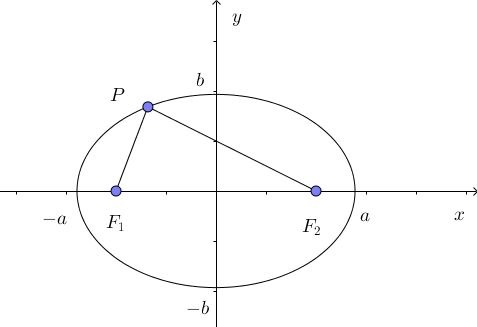
\includegraphics[width=10cm]{images/ellipse.jpg}
\end{figure}

An ellipse is mathematically defined by choosing two points $F_1$ and $F_2$, each of which is called a focus, and then drawing a curve through points for which $PF_1+PF_2$ is constant. 

The major axis is the longest distance through the centre between points on the ellipse. Semi-major axis is the distance $a$. The minor axis is the shortest distance. Semi-minor axis is the distance $b$. Eithr focus of the ellipse is located at a distance $c$ from the centre of ellipse, where $a^2=b^2+c^2$.

The eccentricity of an ellipse is defined as $e=\dfrac{c}{a}$, which describes the general shape of the ellipse. For a circle, $c=0$. Higher values of eccentricity correspond to longer and thinner ellipses. The range of values of the eccentricity for an ellipse is $0<e<1$.

\textbf{Aphelion}: point where the planet is the farthest away from the Sun (for object in orbit around Earth, this point is called the \textbf{apogee}), distance = $a+c$

\textbf{Perihelion}: point where the planet is the nearest to the Sun (for object in orbit around Earth, this point is called the \textbf{perigee}), distance = $a-c$
\end{proof}
\pagebreak

\begin{thrm}{Kepler's 2nd Law}{}
A line joining a planet and the Sun sweeps out equal areas during equal intervals of time.
\end{thrm}

\begin{proof}
Kepler's 2nd law is a consequence of the conservation of angular momentum.

By the law of conservation of angular momentum, 
\[ L = rp = mr^2\omega = mr^2\odv{\theta}{t} \]

Area of a small sector $\dd{A}$ swept out by the radial line is given by 
\[ \dd{A} = \frac{1}{2}r^2\dd{\theta} = \frac{1}{2}r^2\odv{\theta}{t}\dd{t} = \frac{1}{2}\frac{L}{m}\dd{t} \implies A=\frac{1}{2}\frac{Lt}{m} \]
Hence for constant $t$, $A$ is constant.
\end{proof}
\pagebreak

\begin{thrm}{Kepler's 3rd Law}{}
The ratio of the square of a planet's period of revolution to the cube of the semi-major axis of its orbit around the Sun is a constant, and this constant is the same for all planets.
\begin{equation}
T^2 = \frac{4\pi^2}{GM}a^3
\end{equation}
where $a$ is the length of the semi-major axis.
\end{thrm}

\begin{proof}
In the case of a circular orbit, gravitational force provides centripetal force for orbit.
\[ mr\omega^2 = G \frac{mM}{r^2} \]
Then, expressing the angular velocity $\omega$ in terms of the orbital period $T$ and then rearranging, results in Kepler's Third Law:

\[ mr\brac{\frac{2\pi}{T}}^2 = G\frac{Mm}{r^2} \implies T^2 = \brac{\frac {4\pi^2}{GM}}r^3 \implies T^2\propto r^3 \]
\end{proof}
\pagebreak

\section{Gravitational potential energy of spherical shell}
Let us consider a uniform spherical shell of mass $M$. Its mass per unit area will be $\sigma = \frac{M}{4\pi R^2}$. Consider a strip of width $R\dd{\theta}$ and radius $R\sin\theta$. The whole shell is made up of such strips.

\begin{figure}[H]
    \centering
    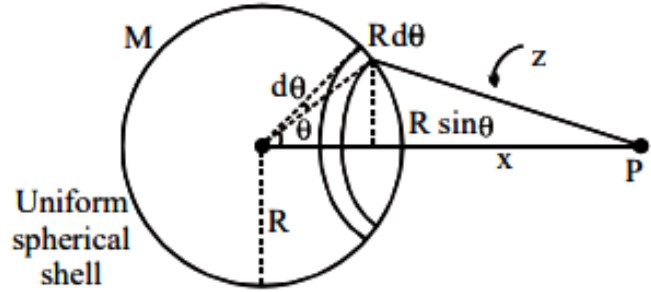
\includegraphics[width=8cm]{images/spherical_shell_gpe.jpg}
\end{figure}

Potential at $P$ due to the ring is given by
\[ \dd{V} = -G\frac{\dd{M}}{z} \] 
\begin{equation}\tag{1}
\dd{V} = -G\frac{2\pi R^2\sin\theta\dd{\theta}}{z}
\end{equation}

Now, 
\[ z = \sqrt{(x-R\cos\theta)^2 + (R\sin\theta)^2} \]
\[ z^2 = x^2 + R^2 - 2xR\cos\theta \]

Differentiating, we get
\[ 2xR\sin\theta=2z\dd{z} \]
\begin{equation}\tag{2}
\sin\theta\dd{\theta} = \frac{z\dd{z}}{xR}
\end{equation}

From (1) and (2),
\[ \dd{V} = -\frac{GM}{2z}\frac{z\dd{z}}{xR} = -\frac{GM}{2xR}\dd{z} \]

\textbf{Case 1: P lies outside the shell}

In this case $x-R \le z \le x-R$. Therefore potential is 
\[ V = -\frac{GM}{2xR}\int_{x-R}^{x+R}\dd{z} = -\frac{GM}{2xR}2R = -\frac{GM}{x} \]

\textbf{Case 2: P lies inside the shell}

In this case $R-x \le z \le x-R$. Therefore potential is 
\[ V=-\frac{GM}{2x}\int_{R-x}^{x+R}\dd{z}=-\frac{GM}{R} \]
\pagebreak

\section{Elliptical orbits and orbital transfers}
To solve problems involving orbital transfers, the key strategy is to work from energy considerations in satellite motion. Recall that the total mechanical energy $E$ of a bound satellite system is $E=-\frac{GMm}{2r}$.

A similar expression for $E$ for elliptical orbits is the same, with $r$ replaced by the semi-major axis of length $a$:
\[ E=-\frac{GMm}{2a} \]
\pagebreak

\section{Effective radial potential}
An orbiting satellite of mass $m$ under the influence of the gravitational field due to the Earth of mass $M$, is at a distance $r$ from the centre of Earth.

Assuming that the system consists of Earth and a satellite and the mass of Earth is many times larger than that of satellite, total energy $U$ of the system is given by 
\[ E_\text{total} = \frac{1}{2}mv_r^2 + \frac{L^2}{2mr^2} - \frac{GMm}{r} \]
where $L$ is angular momentum of satellite, $v_r$ is radial velocity of satellite.

\begin{derivation}
Total energy of a moving satellite m under the influence of the gravitational field due to the Earth of mass M is given by: 
\[ U = E_k+E_p = \frac{1}{2}mv^2 - \frac{GMm}{r} \]
Since the satellite has an ellipsoidal orbit,
\[ v^2 = v_t^2 + v_r^2 \]
Since satellite is in a central force field $\tau=\vb{r}\times\vb{F}=\mathbf{0}$ and $L=mrv_t$.

Therefore, sub into equations and simplifying, 
\[ E_\text{total} = \frac{1}{2}mv_t^2 + \frac{1}{2}mv_r^2 - \frac{GMm}{r} = \boxed{\frac{1}{2}mv_r^2 + \frac{L^2}{2mr^2} - \frac{GMm}{r}} \]
\end{derivation}

Hence \textbf{effective potential} is given by
\[ U_\text{eff} = E_\text{total} - \text{KE}_r = \boxed{\frac{L^2}{2mr^2} - \frac{GMm}{r}} \]

\begin{equation}
U_\text{eff} = \frac{L^2}{2mr^2} - \frac{GMm}{r}
\end{equation}

\chapter{Hydrodynamics}
\section{Fluid Statics}
\begin{thrm}{Pascal's principle}{}
In equilibrium, the pressure in a static varies with height:
\begin{equation}
\dv{P}{y}=-\rho g
\end{equation}

This always holds in equilibrium. For instance, if we squeeze a sealed container of fluid, increasing the pressure locally, then this pressure increase must propagate throughout the entire fluid to maintain $dP/dy = -\rho g$.
\end{thrm}

\begin{thrm}{Archimedes' Principle}{}
An object in a fluid experiences an upward buoyant force due to the different pressures on its top and bottom sides. The force is equal in magnitude to the weight of the fluid displaced.
\end{thrm}

\subsection{Surface tension}
Surface tension and the associated energy, capillary pressure.
\pagebreak

\section{Fluid Mechanics}
Steady flow is where every fluid particle arriving at a given point has the same velocity.

Viscosity is the degree of internal friction; resistance that 2 adjacent layers of the fluid have to move relative to each other.

Ideal fluid flow:
\begin{enumerate}
    \item Non-viscous
    \item Steady
    \item Incompressible
    \item Irrotational
\end{enumerate}

\begin{thrm}{Equation of continuity}{}
This equation says that the flow of fluid through a tube of changing cross section is constant.
\begin{equation}
A_1 v_1 = A_2 v_2
\end{equation}
\end{thrm}

\begin{derivation}
Conservation of mass

Consider the case of a fluid moving from a region of cross-sectional area $A_1$ to a region of area $A_2$. Since the fluid is incompressible, the same amount of it leaves each region and enters the other region during the same time interval.

Volume of fluid that flows into the tube across $A_1$ in time interval $\Delta t$ is \[ \Delta V_1=A_1v_1\Delta t \] 
Hence the mass of fluid that flows into the tube in time $\Delta t$ is
\[ \Delta m_1 = \rho\Delta V_1 = \rho A_1v_1\Delta t \]
Similarly, the mass of fluid that flows across $A_2$ is
\[ \Delta m_2 = \rho\Delta V_2 = \rho A_2v_2\Delta t \]
Equating the two masses,
\[ \Delta m_1 = \Delta m_2 \implies \boxed{A_1v_1=A_2v_2} \]
\end{derivation}

\begin{thrm}{Bernoulli's equation}{}
\begin{equation}
P_1 + \frac{1}{2}\rho {v_1}^2 + \rho gy_1 = P_2 + \frac{1}{2}\rho {v_2}^2 + \rho gy_2 = \text{constant}
\end{equation}
\end{thrm}

\begin{derivation}
Conservation of energy

% https://www.khanacademy.org/science/physics/fluids/fluid-dynamics/a/what-is-bernoullis-equation
\end{derivation}

\subsection{Viscosity}


\begin{thrm}{Poiseuille's Law}{}
\begin{equation}
P_1 - P_2 = 8\frac{Q\eta L}{\pi R^4}
\end{equation}
where $Q$ is the flow rate, $\eta$ is the coefficient of viscosity.
\end{thrm}

